\section{State of Art models}

\begin{frame}{Overview of the architecture and workflow of general EEG-FM Encoder}

    \begin{figure}
        \centering
        \includegraphics[width=0.95\linewidth]{figures/eegfm_encoder.png}
        Source: \cite{lai2025simplerevieweegfoundation}
    \end{figure}

\end{frame}

\begin{frame}{Model Sizes of EEG Foundation Models}
    \begin{figure}
        \centering
        \footnotesize
        % Requires:
% \usepackage{pgfplots}
% \pgfplotsset{compat=1.18}

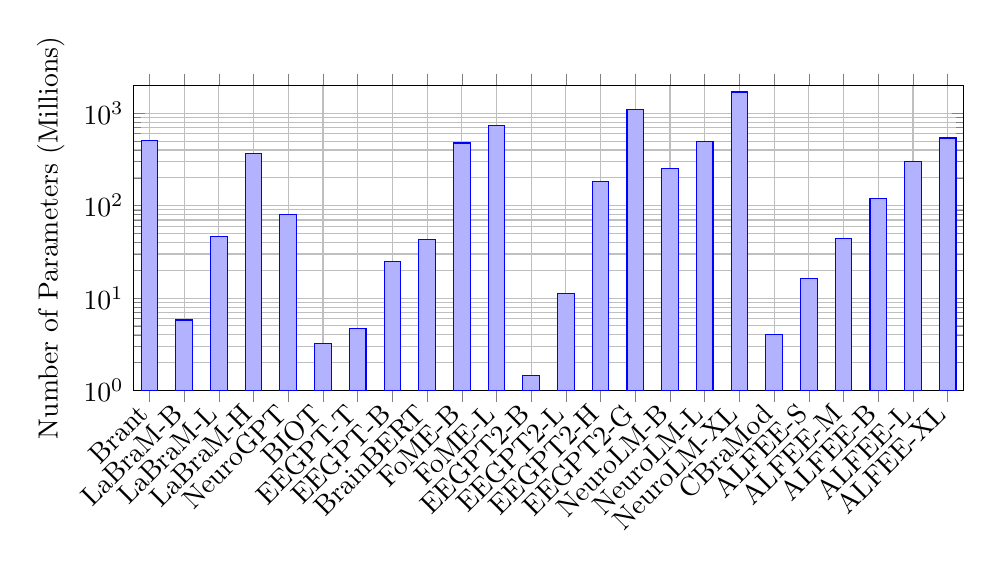
\begin{tikzpicture}
    \begin{axis}[
            ybar,
            width=\linewidth,
            height=0.45\linewidth,
            ylabel={Number of Parameters (Millions)},
            symbolic x coords={
                    Brant,
                    LaBraM-B, LaBraM-L, LaBraM-H,
                    NeuroGPT,
                    BIOT,
                    EEGPT-T, EEGPT-B,
                    BrainBERT,
                    FoME-B, FoME-L,
                    EEGPT2-B, EEGPT2-L, EEGPT2-H, EEGPT2-G,
                    NeuroLM-B, NeuroLM-L, NeuroLM-XL,
                    CBraMod,
                    ALFEE-S, ALFEE-M, ALFEE-B, ALFEE-L, ALFEE-XL
                },
            xtick=data,
            x tick label style={rotate=45, anchor=east},
            ymode=log,
            ymin=1,
            ymax=2000,
            log basis y={10},
            bar width=6pt,
            enlarge x limits=0.02,
            grid=both,
        ]

        \addplot coordinates {
                (Brant,505.69)

                (LaBraM-B,5.8)
                (LaBraM-L,46)
                (LaBraM-H,369)

                (NeuroGPT,79.53)
                (BIOT,3.2)

                (EEGPT-T,4.7)
                (EEGPT-B,25)

                (BrainBERT,43.18)

                (FoME-B,476.3)
                (FoME-L,744.8)

                (EEGPT2-B,1.46)
                (EEGPT2-L,11.29)
                (EEGPT2-H,183.8)
                (EEGPT2-G,1090)

                (NeuroLM-B,254)
                (NeuroLM-L,500)
                (NeuroLM-XL,1696)

                (CBraMod,4.0)

                (ALFEE-S,16.3)
                (ALFEE-M,44.3)
                (ALFEE-B,120)
                (ALFEE-L,300)
                (ALFEE-XL,540)
            };

    \end{axis}
\end{tikzpicture}

    \end{figure}

\end{frame}


\begin{frame}{Pretraining vs Downstream Data Scale}
    \begin{figure}
        \centering
        \footnotesize
        % Requires:
% \usepackage{pgfplots}
% \pgfplotsset{compat=1.18}

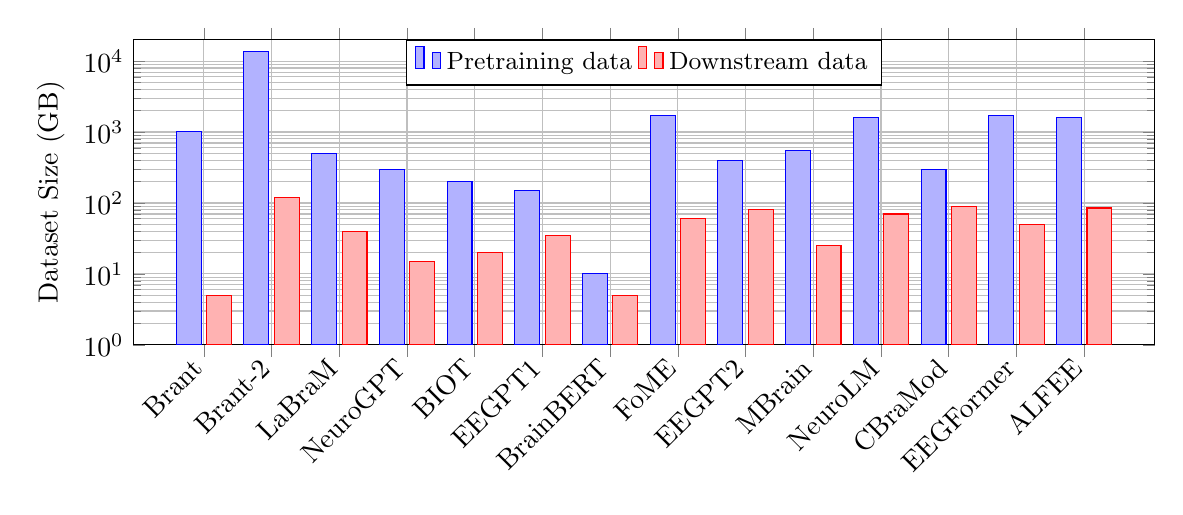
\begin{tikzpicture}
    \begin{axis}[
            ybar,
            width=\linewidth,
            height=0.45\linewidth,
            ylabel={Dataset Size (GB)},
            ymode=log,
            ymin=1,
            x=0.86cm,
            ymax=20000,
            log basis y={10},
            symbolic x coords={
                    Brant,
                    Brant-2,
                    LaBraM,
                    NeuroGPT,
                    BIOT,
                    EEGPT1,
                    BrainBERT,
                    FoME,
                    EEGPT2,
                    MBrain,
                    NeuroLM,
                    CBraMod,
                    EEGFormer,
                    ALFEE
                },
            xtick=data,
            x tick label style={rotate=45, anchor=east},
            bar width=9pt,
            enlarge x limits=0.08,
            grid=both,
            legend style={
                    at={(0.5,0.85)},
                    anchor=south,
                    legend columns=2,
                    font=\small
                }
        ]

        % Pretraining dataset size (GB, approximate from Table I / text)
        \addplot coordinates {
                (Brant,1010)
                (Brant-2,13790)
                (LaBraM,500)
                (NeuroGPT,300)
                (BIOT,200)
                (EEGPT1,150)
                (BrainBERT,10)
                (FoME,1700)
                (EEGPT2,400)
                (MBrain,550)
                (NeuroLM,1600)
                (CBraMod,300)
                (EEGFormer,1700)
                (ALFEE,1600)
            };
        \addlegendentry{Pretraining data}

        % Downstream dataset size (GB-equivalent, indicative)
        \addplot coordinates {
                (Brant,5)
                (Brant-2,120)
                (LaBraM,40)
                (NeuroGPT,15)
                (BIOT,20)
                (EEGPT1,35)
                (BrainBERT,5)
                (FoME,60)
                (EEGPT2,80)
                (MBrain,25)
                (NeuroLM,70)
                (CBraMod,90)
                (EEGFormer,50)
                (ALFEE,85)
            };
        \addlegendentry{Downstream data}

    \end{axis}
\end{tikzpicture}

    \end{figure}
\end{frame}






\begin{frame}{Binary Heatmap of Pretraining Objectives}
    \begin{figure}
        \centering
        \footnotesize
        \begin{tikzpicture}
    \begin{axis}[
            width=\linewidth,
            height=0.35\linewidth,
            ylabel={Reconstruction Objective},
            ytick={0,...,5},
            yticklabels={
                    $L_{op}$,
                    $L_{pe}$,
                    $L_{A}$,
                    $L_{\phi}$,
                    $L_{nnt}$,
                    $L_{eq}$
                },
            xtick={0,...,13},
            xticklabels={
                    Brant,
                    Brant-2,
                    LaBraM,
                    NeuroGPT,
                    BIOT,
                    EEGPT1,
                    BrainBERT,
                    FoME,
                    EEGPT2,
                    MBrain,
                    NeuroLM,
                    CBraMod,
                    EEGFormer,
                    ALFEE
                },
            tick label style={font=\scriptsize},
            x tick label style={rotate=45, anchor=east},
            colormap={themecolors}{
                    color=(white)
                    color=(MyAccent)
                },
            point meta min=0,
            point meta max=1,
            enlargelimits=false,
        ]

        \addplot [
            matrix plot*,
            mesh/cols=14,
            point meta=explicit,
            draw=black,
            line width=0.2pt,
        ] table[meta index=2] {
                x y c
                % y=0: Lop (FIXED — all models use reconstruction)
                0 0 1
                1 0 1
                2 0 1
                3 0 1
                4 0 1
                5 0 1
                6 0 1
                7 0 1
                8 0 1
                9 0 1
                10 0 1
                11 0 1
                12 0 1
                13 0 1

                % y=1: Lpe
                0 1 0
                1 1 0
                2 1 0
                3 1 1
                4 1 1
                5 1 0
                6 1 1
                7 1 0
                8 1 0
                9 1 0
                10 1 0
                11 1 0
                12 1 0
                13 1 0

                % y=2: LA
                0 2 0
                1 2 0
                2 2 1
                3 2 0
                4 2 0
                5 2 0
                6 2 0
                7 2 0
                8 2 0
                9 2 0
                10 2 0
                11 2 0
                12 2 0
                13 2 0

                % y=3: Lphi
                0 3 0
                1 3 0
                2 3 1
                3 3 0
                4 3 0
                5 3 0
                6 3 0
                7 3 0
                8 3 0
                9 3 0
                10 3 1
                11 3 0
                12 3 0
                13 3 0

                % y=4: Lnnt
                0 4 0
                1 4 0
                2 4 1
                3 4 0
                4 4 0
                5 4 0
                6 4 0
                7 4 0
                8 4 0
                9 4 0
                10 4 1
                11 4 0
                12 4 1
                13 4 0

                % y=5: Leq
                0 5 0
                1 5 0
                2 5 1
                3 5 0
                4 5 0
                5 5 0
                6 5 0
                7 5 0
                8 5 0
                9 5 0
                10 5 1
                11 5 0
                12 5 1
                13 5 0
            };

    \end{axis}
\end{tikzpicture}

    \end{figure}

    Reconstruction tasks used during pretraining for different models: {\color{MyAccent}\boldmath$L_{op}$}, patch reconstruction; {\color{MyAccent}\boldmath$L_{pe}$}, embedding reconstruction; {\color{MyAccent}\boldmath$L_{A}$/$L_{\phi}$}, Fourier amplitude/phase regression; {\color{MyAccent}\boldmath$L_{nnt}$/$L_{eq}$}, neural-tokenizer codebook/commitment prediction.

\end{frame}


\begin{frame}{Downstream Task Performance Summary}
    \centering
    \setlength{\tabcolsep}{3pt}
    \renewcommand{\arraystretch}{1.0}
    \scalebox{1.7}{%
        \begingroup\tiny
        \begin{tabular}{l l l c}
            \toprule
            \textbf{Model} & \textbf{Task}         & \textbf{Dataset} & \textbf{Accuracy (\%)}         \\
            \midrule
            \multicolumn{4}{l}{\textit{Clinical Applications \cite{eegbench2024}}}                     \\
            \midrule
            LaBraM         & Abnormal detection    & TUAB             & 83.8                           \\
            BENDR          & Epilepsy detection    & Epilepsy         & 74.0                           \\
            NeuroGPT       & Epilepsy detection    & Epilepsy         & 73.4                           \\
            LaBraM         & OCD classification    & OCD              & 74.0                           \\
            LaBraM         & Stress classification & Real-world       & 90.5                           \\
            \midrule
            \multicolumn{4}{l}{\textit{BCI Applications - Cross-subject Transfer \cite{adabrain2025}}} \\
            \midrule
            CBraMod        & Mental workload       & EEGMAT           & 88.9                           \\
            LaBraM         & Mental workload       & EEGMAT           & 85.8                           \\
            CBraMod        & Sleep staging         & SHHS             & 73.5                           \\
            BIOT           & Sleep staging         & SHHS             & 72.2                           \\
            \midrule
            \bottomrule
        \end{tabular}%
        \endgroup
    }

\end{frame}

\begin{frame}{Current Challenges in EEG Foundation Models}

    \begin{block}{Preprocessing \& Normalization}
        Minimal preprocessing; unclear impact of noise, outliers, and data variability.
    \end{block}

    \begin{block}{Evaluation \& Benchmarking}
        No common benchmarks; limited out-of-distribution and few-shot/zero-shot testing.
    \end{block}

    \begin{block}{Long-Term Context Modeling}
        Difficulty handling diverse timescales (ms ERPs to hours-long sleep stages).
    \end{block}

    \begin{block}{Trustworthiness \& Interpretability}
        No focus on interpretability; essential for clinical trust in high-stakes diagnoses.
    \end{block}

\end{frame}